\chapter{Konvoi}

\section{Motivation}
Die Aufgabe für den ersten Workshop sollte hauptsächlich zum Einstieg in die Serie dienen. Bekannte Elemente wie z.B. der Linienfolgeroboter, der als Anleitung in dem Standardbaukastens beiliegt. sollen hier verwendet werden können, um die Aufgabenstellung zu lösen. Darum wurde als Aufgabe der Konvoi gewählt. Dahinter verbirgt sich einfach gesprochen, ein klassischer Linienfolgeroboter, der in Verbindung mit einer Abstandsmesser zusammen mit dem vorausfahrenden Roboter zu einem Konvoi wird. Die Aufgabe hilft den Teams als Aufwärmübung. Das Equipment wird dabei auf etwaige Fehler überprüft, das Team kann sich einspielen und jeder kann in seine Rolle finden.
    
Um die Sache ein wenig ansprechender zu gestalten und ein wenig der Bezug zu der Realität herzustellen wurde die Aufgabenstellung in eine Hintergrundgeschichte mit Fahrassistenzsystemen verpackt.
\clearpage
\section{Hintergrundgeschichte}
Ein Verband von Fahrzeugen muss Hilfsgüter nach einer Naturkatastrophe im Konvoi über eine Passstraße steuern. Um keine Menschen auf dem unsicheren Terrain zu gefährden, muss ein führerloses Transportsystem eingesetzt werden, um die Güter zu den von der Außenwelt abgeschnitten Menschen zu bringen. Doch leider ist ein Fahrzeug aus dem Konvoi gestohlen worden und es muss von Euch schnell aus Ersatzteilen ein Neues gebaut werden.

\begin{capfigure}[Konvoi]
	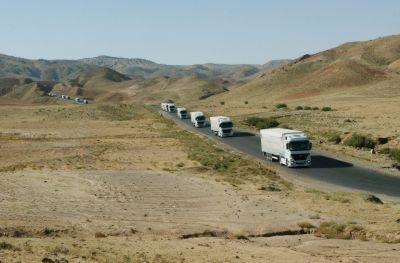
\includegraphics[width=12cm]{images/konvoi}
\end{capfigure}
\section{Aufgabenstellung}
Bauen Sie ein Fahrzeug aus den gegebenen Teilen, welches folgende Fähigkeiten hat:

\begin{itemize}
	\item Es soll einem vorgegebenen Pfad folgen, ohne ihn zu verlassen
	\item Es soll einen definierten Abstand zum führenden Fahrzeug einhalten
\end{itemize}

Achtung! Das Führungsfahrzeug wird bei jedem Transport je nach Gefahr den Pfad unterschiedlich schnell entlang fahren

\begin{capfigure}[Strecke]
	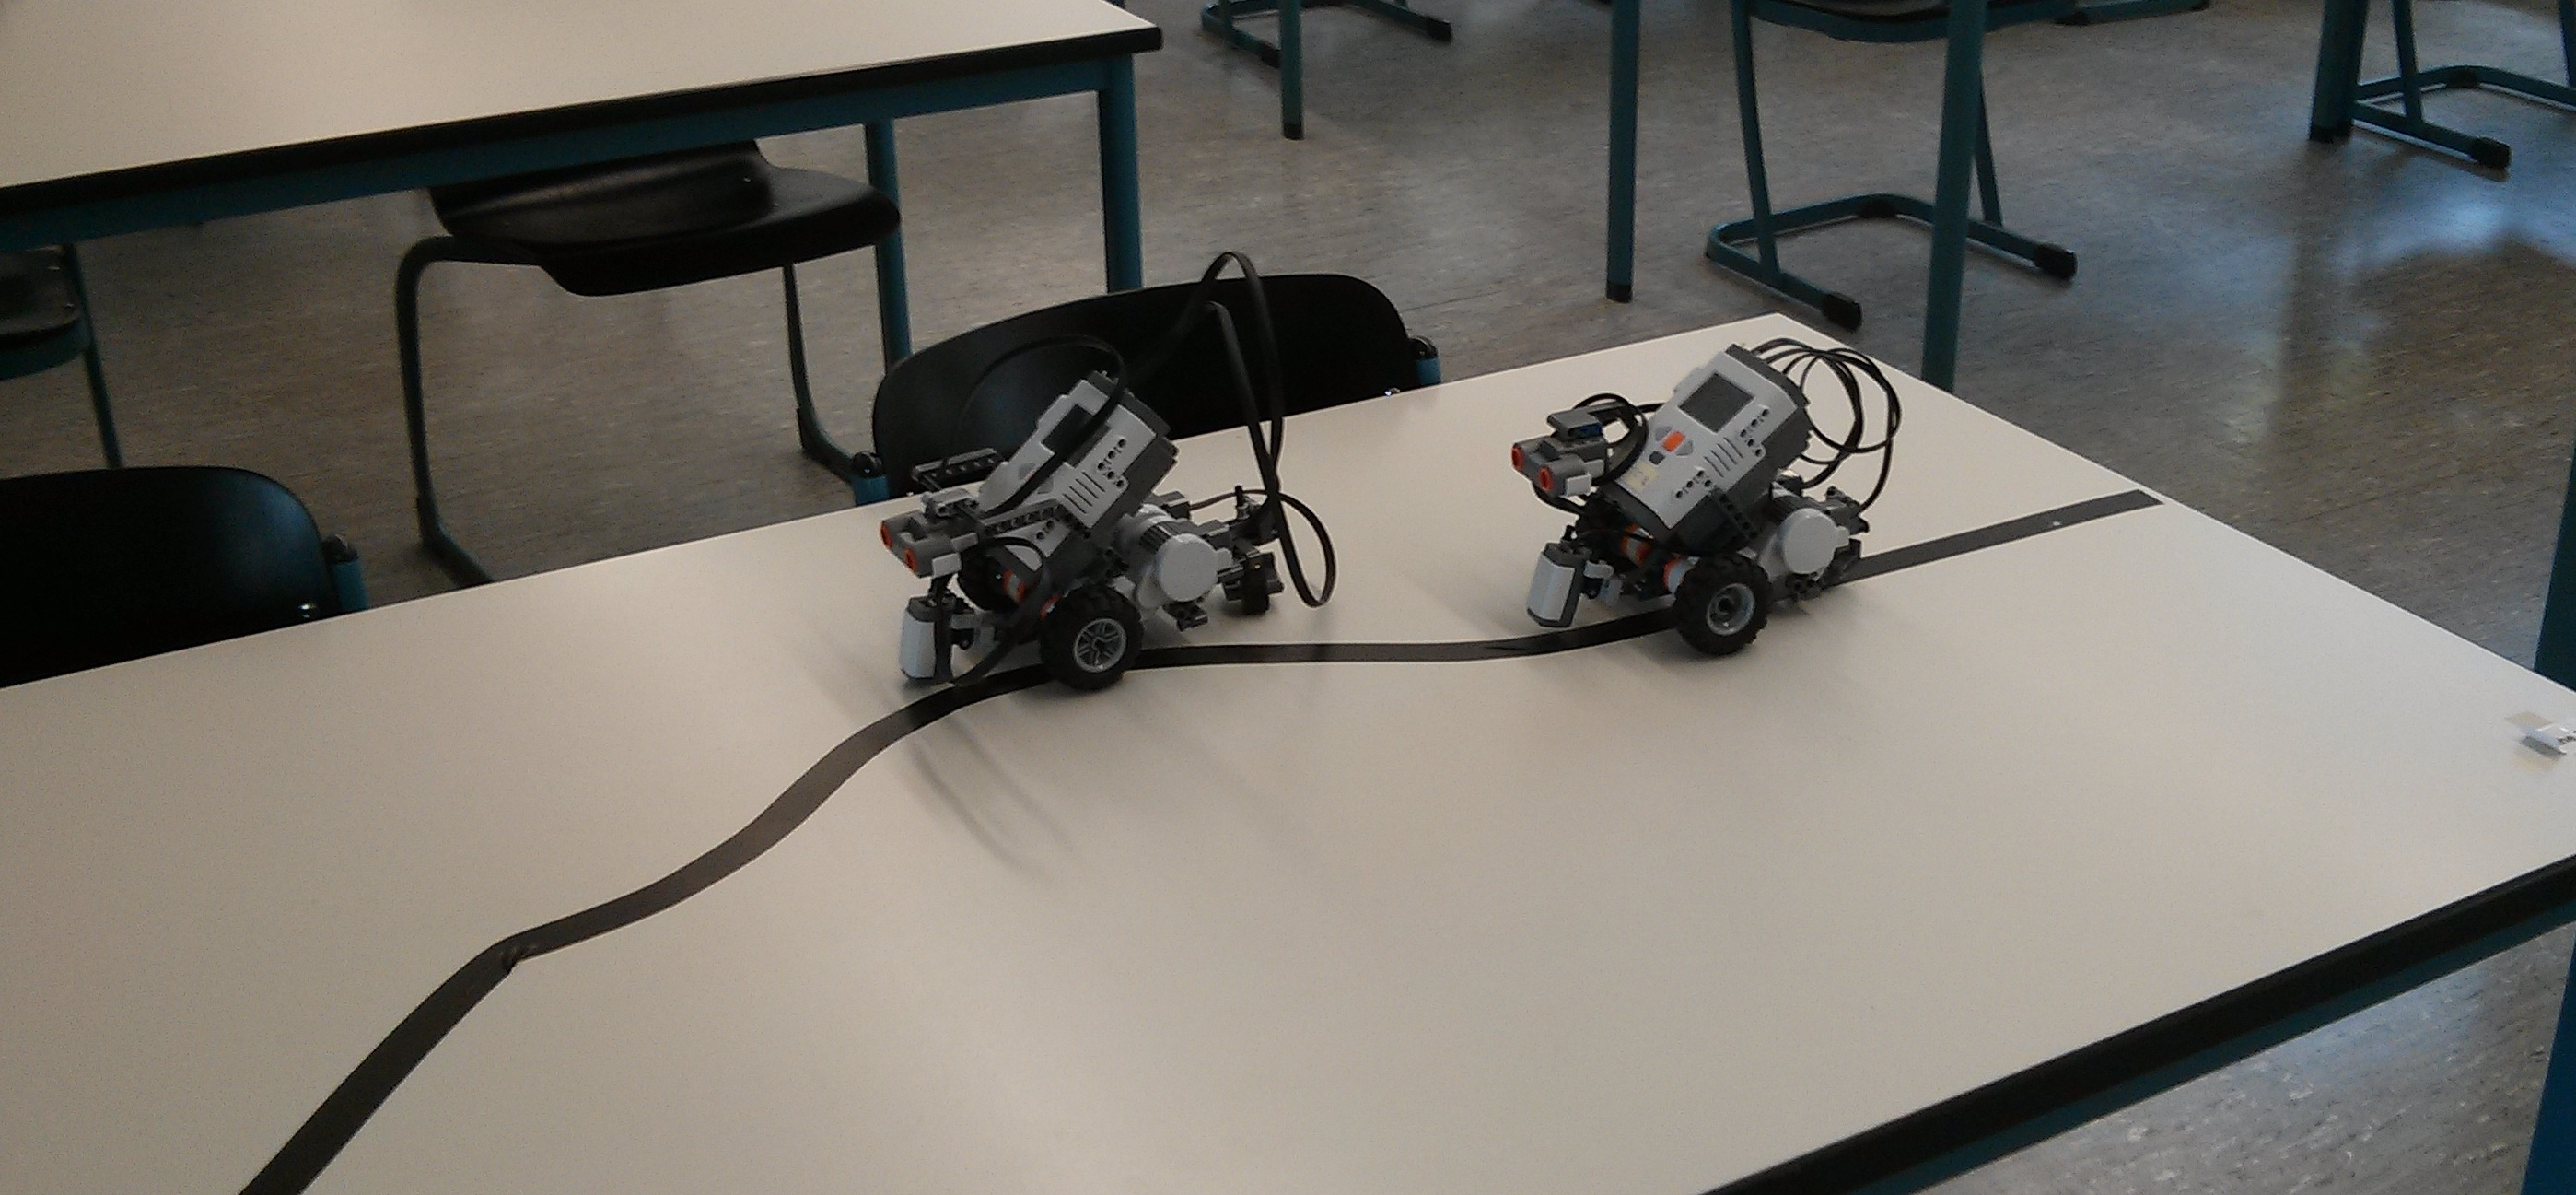
\includegraphics[width=10cm]{images/fotokonvoi}
\end{capfigure}
    
\section{Lösung}
Die Lösung besteht aus einem Teil für die Schüler und einem Teil für die Studenten.
    
\subsection{Führungsfahrzeug}
Das Führungsfahrzeug besteht aus dem Standardlinienfolger des Baukastens. Er benötigt im Gegensatz zum Folger keinen Ultraschallsensor. Um die ein Hardcoding der Schüler bei der Abstandsregelung auszuschließen, wurde dem Führungsfahrzeug eine von einem Zufallsgeschwindigkeit spendiert. In einem zufällig langen Intervall wechselt es die Geschwindigkeit und bleibt sogar zeitweise ganz stehen. 
      
      
      \begin{capfigure}[Standardmodell]
	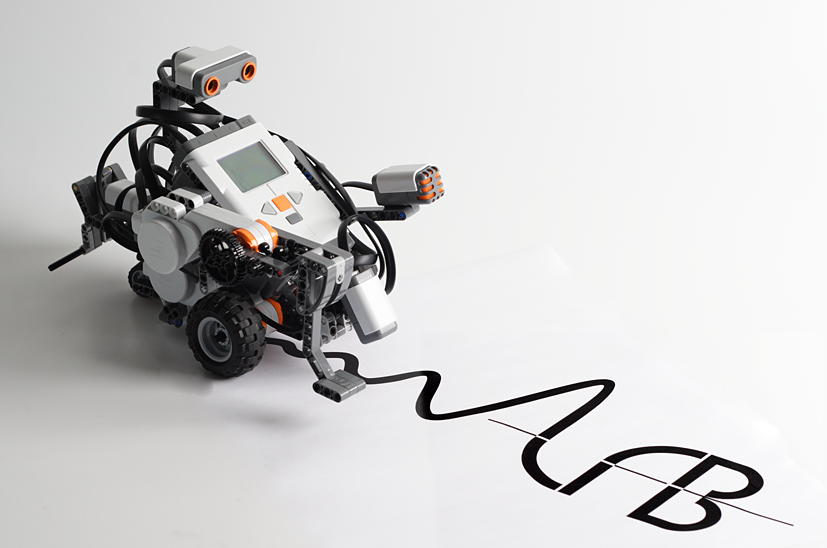
\includegraphics[width=8cm]{images/robostand.png}
      \end{capfigure}
     
Die Lösung kann auch als Video auf der DVD betrachtet werden. Materialien befinden sich unter: \textit{Lösungen/Konvoi}.
    
\subsection{Folger}
Der Aufbau des Folgers ist dem des Führungsfahrzeugs ähnlich. Lediglich der Utraschallsensor ist noch zusätzlich am Fahrzeug angebracht, damit der Abstand detektiert werden kann.

Der Code ist ebenfalls zu dem Führungsfahrzeug sehr ähnlich: Der Linienfolgealgorithmus stimmt überein. An Stelle der zufallsgesteuerten Geschwindigkeit, ist eine einfache 2 Punkt Abstandsregelung implementiert. Sie regelt die Geschwindigkeit in Abhängigkeit zum Abstand
    
\section{Variation in der Aufgabenstellung}
\subsection{Wahl des Linienfolgertyps}
Die Anforderung kann so gestaltet werden, dass eine Zweipunktregelung, wie sie in unserer Musterlösung verwendet wurde gegen einen PI-Regler getauscht wird.
    
\subsection{Abstandstandsregelung}
Auch die Abstandsregelung kann von einer Zweipunktregelung in einer kontinuierliche überführt werden. Entgegen der Regelung mit dem Linienfolger ist der Ultraschallsensor des Mindstorms-System unter 20 cm ungenau. Hierzu müsste ein Meridianfilter implementiert werden, was als Lösung für Schüler nicht zumutbar ist.
    
\subsection{Ohne Linienfolger}
Der Roboter könnte ohne Linie einfach versuchen, das vorangegangene Fahrzeug mit Hilfe des Ultraschallsensors anzupeilen und zu folgen.
      
\subsection{Rückwärtsfahren}
Es wäre auch durchaus möglich, das Führungsfahrzeug rückwärts fahren zu lassen. somit müsste der Roboter so konstruiert sein, dass die Linienfolge auch rückwärts funktioniert.
